\documentclass[tikz,border=8pt]{standalone}
% Shared look for every TikZ diagram. Load with % Shared look for every TikZ diagram. Load with % Shared look for every TikZ diagram. Load with \input{../../tools/tikz-style.tex}
\usepackage[T1]{fontenc}
\usepackage{lmodern}
\renewcommand{\sfdefault}{lmr}  % diagrams use the same serif as the text
\usetikzlibrary{arrows.meta, positioning, shapes.geometric, calc, fit, backgrounds}
\definecolor{cblue}{HTML}{4C78A8}
\definecolor{corange}{HTML}{F58518}
\definecolor{cgreen}{HTML}{54A24B}
\definecolor{cred}{HTML}{E45756}
\definecolor{cpurple}{HTML}{B279A2}
\definecolor{cgrey}{HTML}{6B6B6B}
\tikzset{
  every picture/.style={font=\sffamily, line width=1.2pt},
  box/.style={draw=#1, fill=#1!12, rounded corners=4pt, align=center, inner sep=7pt, minimum height=1.1cm},
  box/.default=cgrey,
  arrow/.style={-{Stealth[length=3mm]}, draw=cgrey, line width=1.4pt},
  title/.style={font=\sffamily\bfseries\Large},
  note/.style={font=\sffamily\small, text=cgrey, align=center},
}
\AtBeginDocument{\hyphenpenalty=10000 \exhyphenpenalty=10000}

\usepackage[T1]{fontenc}
\usepackage{lmodern}
\renewcommand{\sfdefault}{lmr}  % diagrams use the same serif as the text
\usetikzlibrary{arrows.meta, positioning, shapes.geometric, calc, fit, backgrounds}
\definecolor{cblue}{HTML}{4C78A8}
\definecolor{corange}{HTML}{F58518}
\definecolor{cgreen}{HTML}{54A24B}
\definecolor{cred}{HTML}{E45756}
\definecolor{cpurple}{HTML}{B279A2}
\definecolor{cgrey}{HTML}{6B6B6B}
\tikzset{
  every picture/.style={font=\sffamily, line width=1.2pt},
  box/.style={draw=#1, fill=#1!12, rounded corners=4pt, align=center, inner sep=7pt, minimum height=1.1cm},
  box/.default=cgrey,
  arrow/.style={-{Stealth[length=3mm]}, draw=cgrey, line width=1.4pt},
  title/.style={font=\sffamily\bfseries\Large},
  note/.style={font=\sffamily\small, text=cgrey, align=center},
}
\AtBeginDocument{\hyphenpenalty=10000 \exhyphenpenalty=10000}

\usepackage[T1]{fontenc}
\usepackage{lmodern}
\renewcommand{\sfdefault}{lmr}  % diagrams use the same serif as the text
\usetikzlibrary{arrows.meta, positioning, shapes.geometric, calc, fit, backgrounds}
\definecolor{cblue}{HTML}{4C78A8}
\definecolor{corange}{HTML}{F58518}
\definecolor{cgreen}{HTML}{54A24B}
\definecolor{cred}{HTML}{E45756}
\definecolor{cpurple}{HTML}{B279A2}
\definecolor{cgrey}{HTML}{6B6B6B}
\tikzset{
  every picture/.style={font=\sffamily, line width=1.2pt},
  box/.style={draw=#1, fill=#1!12, rounded corners=4pt, align=center, inner sep=7pt, minimum height=1.1cm},
  box/.default=cgrey,
  arrow/.style={-{Stealth[length=3mm]}, draw=cgrey, line width=1.4pt},
  title/.style={font=\sffamily\bfseries\Large},
  note/.style={font=\sffamily\small, text=cgrey, align=center},
}
\AtBeginDocument{\hyphenpenalty=10000 \exhyphenpenalty=10000}

\begin{document}
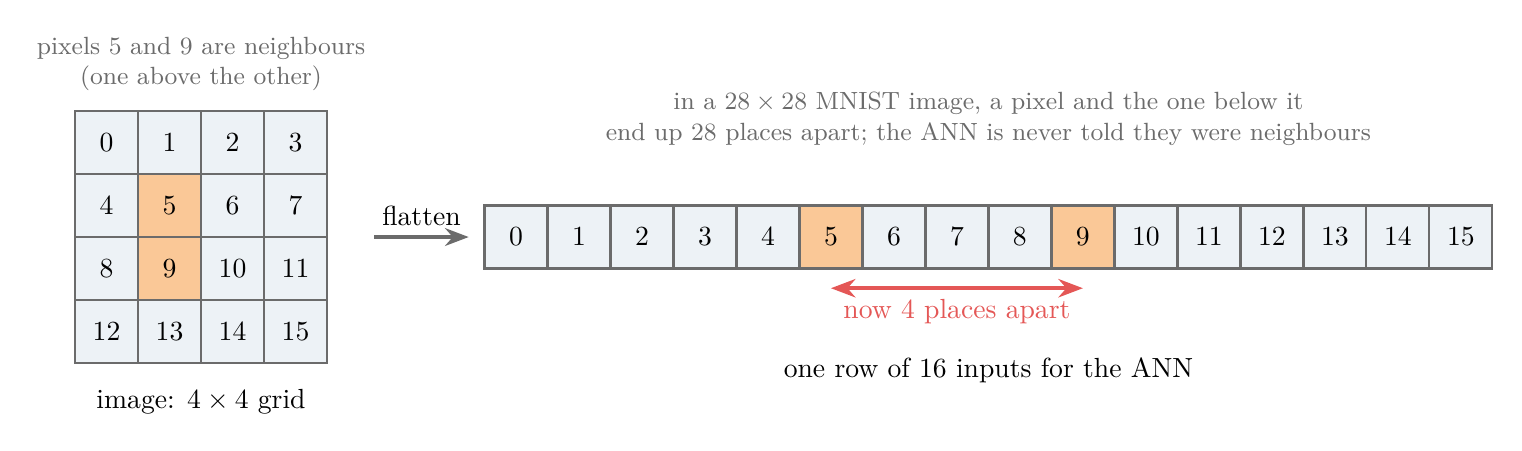
\begin{tikzpicture}[every node/.append style={font=\sffamily}]
  \foreach \r in {0,...,3}{\foreach \c in {0,...,3}{
    \pgfmathtruncatemacro{\k}{4*\r+\c}
    \pgfmathsetmacro{\hl}{(\k==5 || \k==9) ? 1 : 0}
    \ifdim\hl pt=1pt \def\col{corange!45}\else\def\col{cblue!10}\fi
    \node[draw=cgrey, line width=0.8pt, minimum size=0.8cm, fill=\col] at (\c*0.8,-\r*0.8) {\k};
  }}
  \node[below] at (1.2,-3.0) {image: $4 \times 4$ grid};
  \node[note, align=center] at (1.2,1.0) {pixels 5 and 9 are neighbours\\(one above the other)};
  \draw[arrow] (3.4,-1.2) -- (4.6,-1.2) node[midway, above] {flatten};
  \foreach \k in {0,...,15}{
    \pgfmathsetmacro{\hl}{(\k==5 || \k==9) ? 1 : 0}
    \ifdim\hl pt=1pt \def\col{corange!45}\else\def\col{cblue!10}\fi
    \node[draw=cgrey, line width=0.8pt, minimum size=0.8cm, fill=\col] at (5.2+\k*0.8,-1.2) {\k};
  }
  \draw[cred, line width=1.3pt, {Stealth}-{Stealth}] (5.2+5*0.8,-1.85) -- (5.2+9*0.8,-1.85) node[midway, below, text=cred] {now 4 places apart};
  \node[below] at (11.2,-2.6) {one row of 16 inputs for the ANN};
  \node[note, align=center] at (11.2,0.3) {in a $28 \times 28$ MNIST image, a pixel and the one below it\\end up 28 places apart; the ANN is never told they were neighbours};
\end{tikzpicture}
\end{document}
